%
% teil2.tex -- Beispiel-File für teil2
%
% (c) 2020 Prof Dr Andreas Müller, Hochschule Rapperswil
%

\section{L\"osungsmethoden}
\rhead{L\"osungsmethoden}

In diesem Abschnitt werden mehrere Algorithmen zur Berechnung der Matrizenmultiplikation vorgestellt, auch werden Libraries zur automatisierten Verwendung von vordefinierten Algorithmen gezeigt.

\subsection{Standard Algorithmus}

Der Standard Methode kann im Algorithmus \ref{multiplikation:alg:smm} entnommen werden.
Hierf\"ur wurde die Gleichung \eqref{multiplikation:eq:MM} direkt implementiert.
Die \texttt{For i} Schleife iteriert \"uber alle Zeilen der $\mathbf{A}$ Matrix, die \texttt{For j} Schleife iteriert \"uber alle Spalten der $\mathbf{B}$ Matrix und die \texttt{For k} Schleife iteriert \"uber alle Eintr\"age dieser Zeilen bzw. Spalten.

\begin{algorithm}\caption{Matrix Multiplication}
	\label{multiplikation:alg:smm}
	\setlength{\lineskip}{7pt}
	\begin{algorithmic}[1]
		\Function{MM}{$\textbf{A}, \textbf{B}$}
		\State $sum \gets 0$
		\State $n \gets columns(\textbf{A}) == rows(\textbf{B})$
		\State $m \gets rows(\textbf{A})$
		\State $p \gets columns(\textbf{B})$
		\State $\textbf{C} \gets zeros(m,p)$
		\For{$i = 0,1,2 \dots,m-1$}
		\For{$j = 0,1,2 \dots,p-1$}
		\State $sum \gets 0$
		\For{$k = 0,1,2 \dots,n-1$}
		\State $sum \gets  sum + \textbf{A}[i][k] \cdot \textbf{B}[k][j]$
		\EndFor
		\State $\textbf{C}[i][j] \gets  sum $
		\EndFor
		\EndFor
		\State \textbf{return} $\textbf{C}$
		\EndFunction
	\end{algorithmic}
\end{algorithm}

Die Laufzeit dieser Struktur mit drei \texttt{For} Schleifen ist $\mathcal{O}(n^3)$

\subsubsection{Divide and Conquer Methode}

F\"ur gewisse Algorithmen f\"uhren \textit{Divide and Conquer} Ans\"atze zu markant besseren Laufzeiten.
Das bekannteste Beispiel ist wohl die \textit{Fast Fourier Transform} wobei die Laufzeit von $\mathcal{O}(n^2)$ zu $\mathcal{O}(n \log n)$ verbessert werden kann.

Die Matrizenmultiplikation kann ebenfalls mit solch einem Ansatz berechnet werden.
Zur vereinfachten Veranschaulichung kann die Situation, mit $\mathbf{A}$ und $\mathbf{B}$ der gr\"osse $2^n \times 2^n$ verwendet werden.
Die Matrizen $\mathbf{A}$ und $\mathbf{B}$ werden in jeweils vier Blockmatrizen der gr\"osse $2^{n-1} \times 2^{n-1}$
\begin{equation}
\mathbf{A}\mathbf{B}=
\begin{bmatrix}
\mathbf{A}_{11} & \mathbf{A}_{12}\\
\mathbf{A}_{21} & \mathbf{A}_{22}
\end{bmatrix}
\begin{bmatrix}
\mathbf{B}_{11} & \mathbf{B}_{12}\\
\mathbf{B}_{21} & \mathbf{B}_{22}
\end{bmatrix}
=
\begin{bmatrix}
\mathbf{C}_{11} & \mathbf{C}_{12}\\
\mathbf{C}_{21} & \mathbf{C}_{22}
\end{bmatrix}
\end{equation}
aufgeteilt.
Die Berechnung
\begin{equation}
\mathbf{C}_{ij} = \sum_{k=1}^n \mathbf{A}_{ik} \mathbf{B}_{kj}
\label{multiplikation:eq:MM_block}
\end{equation}
ist identisch zu der Gleichung \eqref{multiplikation:eq:MM}, wobei hier f\"ur die Multiplikation die Matrizenmultiplikation verwendet wird.

Der Algorithmus \ref{multiplikation:alg:devide_mm} zeigt den \textit{Divide and Conquer} Ansatz,
Der Grundstruktur dieser Methode besteht aus dem rekursiven Aufruf der Funktion mit den erzeugten Blockmatrizen.
Der rekursive Aufruf wird bis zu der Gr\"osse der Matrizen von $N = 2 \times 2$ durchgef\"uhrt.
\begin{algorithm}\caption{Divide and Conquer Matrix Multiplication}
	\setlength{\lineskip}{7pt}
	\label{multiplikation:alg:devide_mm}
	\begin{algorithmic}
		\Function{MM}{$\textbf{A}, \textbf{B}, n$}
		\If{$n = 2$}
		\State  $ \mathbf{C} \gets zeros(n, n)$
		\State  $C[0, 0] \gets  A[0][0]\cdot B[0][0]+A[0][1]\cdot B[1][0]$
		\State  $C[0, 1] \gets  A[0][0]\cdot B[0][1]+A[0][1]\cdot B[1][1]$
		\State  $C[1, 0] \gets  A[1][0]\cdot B[0][0]+A[1][1]\cdot B[1][0]$
		\State  $C[1, 1] \gets  A[1][0]\cdot B[0][1]+A[1][1]\cdot B[1][1]$
		\Else
		\State  $ m \gets n/2$
		\State $\mathbf{A11}, \mathbf{A12}, \mathbf{A21}, \mathbf{A22} \gets \mathbf{A}[:m][:m], \mathbf{A}[:m][m:], \mathbf{A}[m:][:m], \mathbf{A}[m:][m:]$
		\State $\mathbf{B11}, \mathbf{B12}, \mathbf{B21}, \mathbf{B22} \gets \mathbf{B}[:m][:m], \mathbf{B}[:m][m:], \mathbf{B}[m:][:m], \mathbf{B}[m:][m:]$

		\State $\mathbf{C11} \gets \text{MM}(\mathbf{A11}, \mathbf{B11},n) + \text{MM}(\mathbf{A12}, \mathbf{B21},n)$
		\State $\mathbf{C12} \gets \text{MM}(\mathbf{A11},\mathbf{B12},n) + \text{MM}(\mathbf{A12}, \mathbf{B22},n)$
		\State $\mathbf{C21} \gets \text{MM}(\mathbf{A21}, \mathbf{B11},n) + \text{MM}(\mathbf{A22}, \mathbf{B21},n)$
		\State $\mathbf{C22} \gets \text{MM}(\mathbf{A21}, \mathbf{B12},n) + \text{MM}(\mathbf{A22}, \mathbf{B22},n)$
		\State $  C \gets vstack(hstack(C11, C12), hstack(C21, C22))$

		\EndIf
		\State \textbf{return} $\textbf{C}$

		\EndFunction
	\end{algorithmic}
\end{algorithm}

Die Laufzeit dieser rekursiven Funktion kann mit dem \textit{Master Theorem} berechnet werden.
Ohne auf diesen vertieft einzugehen, bestimmt die Anzahl rekursiver Aufrufe der Funktion die Laufzeit.
In diesem Fall wird die Funktion pro Durchlauf acht mal rekursiv aufgerufen, dies f\"uhrt
\begin{equation} \label{multiplikation:eq:laufzeitdac}
	\mathcal{T}(n) =
	\begin{cases}
	1  & \text{if }  n \leq 2\\
	8 \cdot \mathcal{T}(\frac{n}{2}) + n^2  & \text{if }  n > 2
	\end{cases} = \mathcal{O}(n^{\log_2 8}) = \mathcal{O}(n^{3})
\end{equation}
zu einer kubischen Laufzeit.
Die Addition zweier Matrizen $\mathbf{A} + \mathbf{B} = \mathbf{C}$ hat eine Laufzeit von $\mathcal{O}(n^{2})$ und kann neben dem dominierendem Anteil von $\mathcal{O}(n^{3})$ ignoriert werden.
In diesem Fall hat der \textit{Divide and Conquer} Ansatz zu keiner Verbesserung gef\"uhrt.


\subsection{Strassen's Algorithmus}

Strassen's Algorithmus \cite{multiplikation:strassen_1969} beschreibt die Matrizenmultiplikation mit einer Vielzahl von Additionen, Subtraktionen und Multiplikationen.
Die Grundlegenden Terme
\begin{equation} \label{multiplikation:eq:strassen}
\begin{split}
\text{\textbf{P}}   &= (\mathbf{A}_{11} + \mathbf{A}_{22}) \cdot (\mathbf{B}_{11} + \mathbf{B}_{22}) \\
\text{\textbf{Q}}  &= (\mathbf{A}_{21} + \mathbf{A}_{22}) \cdot \mathbf{B}_{11} \\
\text{\textbf{R}} &= \mathbf{A}_{11} \cdot (\mathbf{B}_{12}-\mathbf{B}_{22}) \\
\text{\textbf{S}}  &= \mathbf{A}_{22} \cdot (-\mathbf{B}_{11}+\mathbf{B}_{21}) \\
\text{\textbf{T}}   &= (\mathbf{A}_{11} + \mathbf{A}_{12}) \cdot \mathbf{B}_{22} \\
\text{\textbf{U}}  &= (-\mathbf{A}_{11} + \mathbf{A}_{21}) \cdot (\mathbf{B}_{11} + \mathbf{B}_{12}) \\
\text{\textbf{V}} &= (\mathbf{A}_{12} - \mathbf{A}_{22}) \cdot (\mathbf{B}_{21} + \mathbf{B}_{22})
\end{split}
\end{equation}
aus $\mathbf{A}$ und $\mathbf{B}$, werden f\"ur die Berechnung der Matrix $\mathbf{C}$
\begin{equation} \label{multiplikation:eq:strassen2}
\begin{split}
\mathbf{C}_{11} &= \text{\textbf{P}} + \text{\textbf{S}} - \text{\textbf{T}} + \text{\textbf{V}} \\
\mathbf{C}_{21} &= \text{\textbf{R}} + \text{\textbf{T}} \\
\mathbf{C}_{12} &= \text{\textbf{Q}} + \text{\textbf{S}}\\
\mathbf{C}_{22} &= \text{\textbf{P}} + \text{\textbf{R}} - \text{\textbf{Q}} + \text{\textbf{U}}
\end{split}
\end{equation}
gebraucht.
\begin{algorithm}\caption{Strassen Matrix Multiplication}
	\label{multiplikation:alg:strassen}
	\setlength{\lineskip}{7pt}
	\begin{algorithmic}
		\Function{strassen}{$\textbf{A}, \textbf{B}, n$}
		\If{$n = 2$}
		\State  $ \mathbf{C} \gets zeros((n, n))$
		\State $P  \gets (A[0][0]+A[1][1])\cdot( B[0][0]+B[1][1])$
		\State   $Q  \gets (A[1][0]+A[1][1])\cdot B[0][0]$
		\State   $R  \gets A[0][0]\cdot (B[0][1]-B[1][1])$
		\State   $S  \gets A[1][1]\cdot (B[1][0]-B[0][0])$
		\State   $T  \gets (A[0][0]+A[0][1])\cdot B[1][1]$
		\State   $U  \gets (A[1][0]-A[0][0])\cdot (B[0][0]+B[0][1])$
		\State   $V  \gets (A[0][1]-A[1][1])\cdot (B[1][0]+B[1][1])$
		\State   $C[0][0]  \gets P+S-T+V$
		\State   $C[0][1]  \gets R+T$
		\State   $C[1][0]  \gets Q+S$
		\State   $C[1][1]  \gets P+R-Q+U$
		\Else
		\State  $ m \gets n/2$
		\State $\mathbf{A11}, \mathbf{A12}, \mathbf{A21}, \mathbf{A22} \gets \mathbf{A}[:m][:m], \mathbf{A}[:m][m:], \mathbf{A}[m:][:m], \mathbf{A}[m:][m:]$
		\State $\mathbf{B11}, \mathbf{B12}, \mathbf{B21}, \mathbf{B22} \gets \mathbf{B}[:m][:m], \mathbf{B}[:m][m:], \mathbf{B}[m:][:m], \mathbf{B}[m:][m:]$

		\State $ \mathbf{P} \gets \text{strassen}((\mathbf{A11}+ \mathbf{A22}),(\mathbf{B11}+\mathbf{B22}), m)$
		\State $ \mathbf{Q} \gets \text{strassen}((\mathbf{A21}+ \mathbf{A22}), \mathbf{B11},m)$
		\State $ \mathbf{R} \gets \text{strassen}( \mathbf{A11},(\mathbf{B12}-  \mathbf{B22}),m)$
		\State $ \mathbf{S} \gets \text{strassen}( \mathbf{A22},(\mathbf{B21}-  \mathbf{B11}),m)$
		\State $ \mathbf{T} \gets \text{strassen}((\mathbf{A11}+ \mathbf{A12}), \mathbf{B22},m)$
		\State $ \mathbf{U} \gets \text{strassen}((\mathbf{A21}- \mathbf{A11}),(\mathbf{B11}+\mathbf{B12}),m)$
		\State $ \mathbf{V} \gets \text{strassen}((\mathbf{A12}- \mathbf{A22}),(\mathbf{B21}+\mathbf{B22}),m)$



		\State   $\mathbf{C11}  \gets \mathbf{P+S-T+V}$
		\State   $\mathbf{C12}  \gets \mathbf{R+T}$
		\State   $\mathbf{C21}  \gets \mathbf{Q+S}$
		\State   $\mathbf{C22}  \gets \mathbf{P+R-Q+U}$
		\State $  C \gets vstack(hstack(C11, C12), hstack(C21, C22))$

		\EndIf
		\State \textbf{return} $\textbf{C}$

		\EndFunction
	\end{algorithmic}
\end{algorithm}
Strassens's Methode wird in der Abbildung \ref{multiplikation:fig:strassen} grafisch dargestellt.
\begin{figure}
	\center
	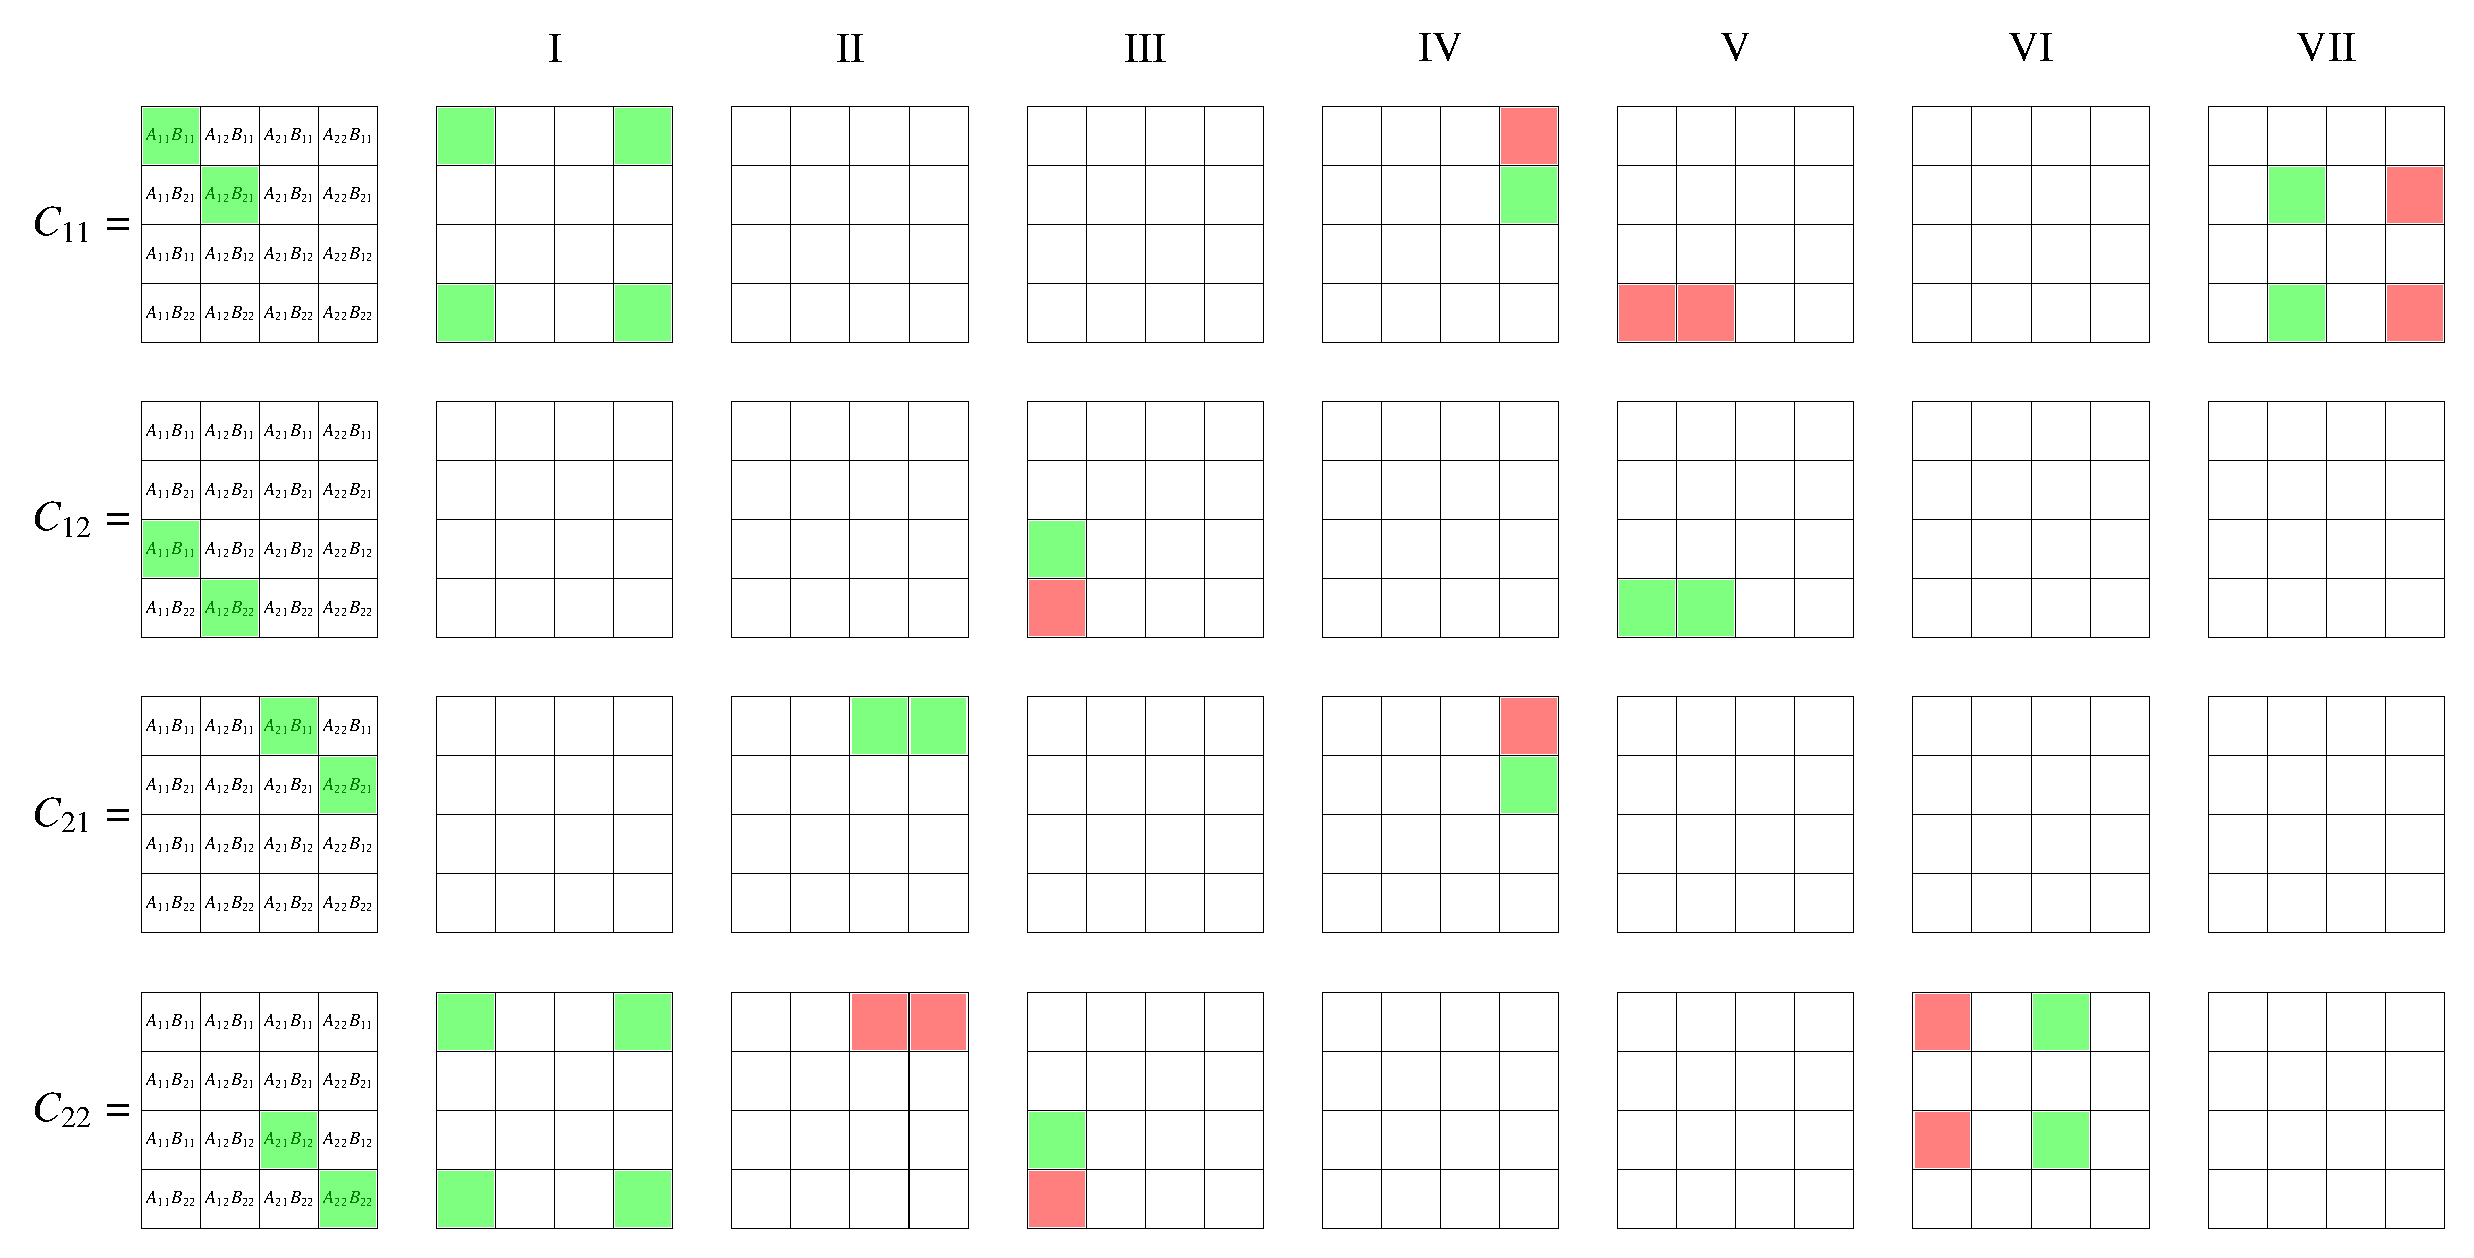
\includegraphics[width=\linewidth]{papers/multiplikation/images/strassen.pdf}
	\caption{Strassen's Algorithmus}
	\label{multiplikation:fig:strassen}
\end{figure}

Die Funktion wird sieben mal rekursiv aufgerufen.
Dies f\"uhrt zu einer Laufzeit von
\begin{equation} \label{multiplikation:eq:laufzeitstrassen}
\mathcal{T}(n) =
\begin{cases}
1  & \text{if }  n \leq 2\\
7 \cdot \mathcal{T}(\frac{n}{2}) + n^2  & \text{if }  n > 2
\end{cases} = \mathcal{O}(n^{\log_2 7}) = \mathcal{O}(n^{2.8074})
\end{equation}
und ist somit schneller als die Standard Methode.

\subsection{Winograd's Algorithmus}

Ein weiterer Ansatz lieferte Shmuel Winograd im Jahre 1968 \cite{multiplikation:winograd_1968}.
Er zeigte einen neuen Algorithmus f\"ur das
\begin{equation}
	\langle x,y \rangle = \sum_{i=1}^{n}x_i y_i
\end{equation}
Skalarprodukt.
F\"ur jeden Vektor berechne
\begin{equation}
	\xi = \sum_{j=1}^{ \lfloor n/2 \rfloor} x_{2j-1} \cdot x_{2j}
\end{equation}
und
\begin{equation}
	\eta = \sum_{j=1}^{ \lfloor n/2 \rfloor} y_{2j-1} \cdot y_{2j}.
\end{equation}
Das Skalarprodukt ist nun geben mit
\begin{equation}
	\langle x,y \rangle =
	\begin{cases}
	 \displaystyle \quad \sum_{j=1}^{ \lfloor n/2 \rfloor} (x_{2j-1} + y_{2j})(x_{2j}+y_{2j-1})-\xi - \eta & \text{if  $n$ is even}\\
	\displaystyle  \quad \sum_{j=1}^{ \lfloor n/2 \rfloor} (x_{2j-1} + y_{2j})(x_{2j}+y_{2j-1})-\xi - \eta + x_n y_n & \text{if  $n$ is odd}.
	\end{cases}
\end{equation}

Angenommen man hat $N$ Vektoren mit welchen man $T$ Skalarprodukte berechnen m\"ochte.
Daf\"ur werden $N\lfloor n/2 \rfloor + T\lfloor (n+1)/2 \rfloor $ Multiplikationen ben\"otigt.
Eine Matrizenmultiplikation mit $\mathbf{A}$ einer $m \times n$ und $\mathbf{B}$ einer $n \times p$ Matrix, entspricht $N=m+p$ Vektoren mit welchen man $T=mp$ Skalarprodukte berechnet.
Dies f\"uhrt zu
\begin{equation}
		(m+p) \left \lfloor \frac{n}{2} \right \rfloor + mp \left \lfloor \frac{n+1}{2} \right \rfloor = \frac{mn}{2} + \frac{pn}{2} + \frac{mpn}{2} + \frac{mp}{2}
\end{equation}
Multiplikationen.
Wenn $m,p,n$ gross werden, dominiert der Term $\frac{mpn}{2}$ und es werden $\frac{mpn}{2}$ Multiplikationen ben\"otigt.
Was im Vergleich zu den $mpn$ Multiplikation der Standard Methode nur die H\"alfte ist.
Die Implementation kann im Algorithmus \ref{multiplikation:alg:winograd} entnommen werden.

\begin{algorithm}\caption{Winograd Matrix Multiplication}
	\setlength{\lineskip}{7pt}
	\label{multiplikation:alg:winograd}
	\begin{algorithmic}
		\Function{Winograd}{$\textbf{A}, \textbf{B}, n$}
		\State  $ m \gets rows(\mathbf{A})$
		\State  $ n \gets columns(\mathbf{A}) == rows(\mathbf{B})$
		\State  $ p \gets columns(\mathbf{B})$
		\State  $ \mathbf{\xi} \gets zeros(m)$
		\State  $ \mathbf{\eta} \gets zeros(p)$


		\For{$i = 0,1,2 \dots,m-1$}
		\For{$j = 0,1,2 \dots,\lfloor n/2 \rfloor-1$}
		\State $\xi[i] \gets \xi[i]+A[i,2 j]A[i,2 j+1]$
		\EndFor
		\EndFor

		\For{$i = 0,1,2 \dots,p-1$}
		\For{$j = 0,1,2 \dots,\lfloor n/2 \rfloor-1$}
		\State $\eta[i] \gets   \eta[i]+B[2 j,i]B[2 j+1,i]$
		\EndFor
		\EndFor

		\If{$n \% 2 == 0$}
		\For{$i = 0,1,2 \dots,m-1$}
		\For{$j = 0,1,2 \dots,p-1$}
		\State $ab \gets 0$
		\For{$k = 0,1,2 \dots,\lfloor n/2 \rfloor-1$}
		\State $ab \gets ab + (A[i,2k]+B[2k+1,j])(A[i,2k+1]+B[2k,j])$
		\EndFor
		\State $C[i,j] \gets ab-\eta[j]-\xi[i]$
		\EndFor
		\EndFor
    \Else
		\For{$i = 0,1,2 \dots,n-1$}
		\For{$j = 0,1,2 \dots,n-1$}
		\State $ab \gets 0$
		\For{$k = 0,1,2 \dots,\lfloor n/2 \rfloor-1$}
		\State $ab \gets ab + (A[i,2k]+B[2k+1,j])(A[i,2k+1]+B[2k,j])$
		\EndFor
		\State $C[i,j] \gets ab-\eta[j]-\xi[i]+A[i,-1]B[-1,j]$
		\EndFor
		\EndFor
		\EndIf
		\State \textbf{return} $\textbf{C}$

		\EndFunction
	\end{algorithmic}
\end{algorithm}

\subsection{Weitere Algorithmen}

\textcolor{red}{TODO: BLAS}

\section{Implementation}
\rhead{Implementation}
\textcolor{red}{TODO: messresultate}

\section{Fazit}
\rhead{Fazit}
